\documentclass[12pt, a4paper]{article}
\usepackage{caption}
\usepackage{graphicx}
\usepackage{listings}
\usepackage{siunitx}
\usepackage{hyperref}
\def\checkmark{\tikz\fill[scale=0.4](0,.35) -- (.25,0) -- (1,.7) -- (.25,.15) -- cycle;}
\usepackage{tikz-network}
\hypersetup{
    colorlinks,
    citecolor=black,
    filecolor=black,
    linkcolor=black,
    urlcolor=black
}
\usepackage{amsmath, amsfonts, amssymb, amsthm}
\renewcommand{\thesubsubsection}{\thesubsection.\alph{subsubsection}}
\title{Algorithms and datastructures\\Exercises}
\date{2022}
\author{Kristoffer Klokker}
\begin{document}
	\maketitle
	\clearpage
	\tableofcontents
	\clearpage
		\setcounter{section}{5}
		\section{Uge}
			\subsection{Indicate the following according to figure 1.}
				\begin{figure}[h!]
					\centering
					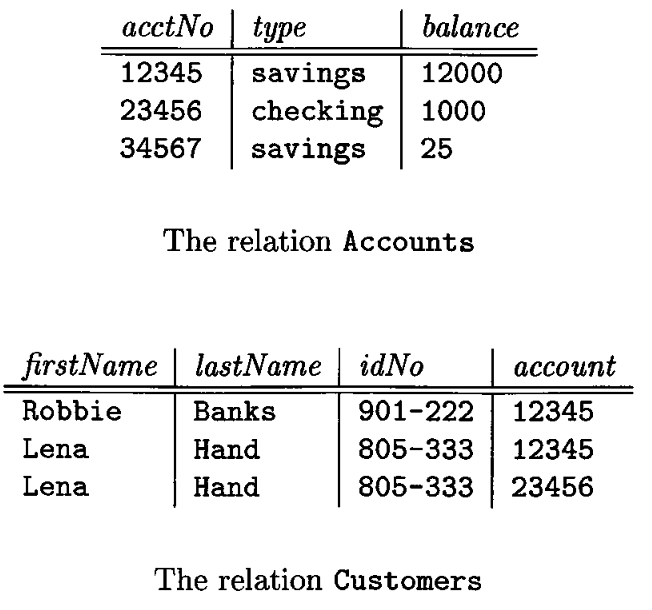
\includegraphics[width=300px]{assets/W6E1.png}
					\caption{Two relations of a banking database}
				\end{figure}
				\subsubsection{The attributes of each realtion}
					Accounts: $acctNo$, $type$, $balance$\\
					Customers: $firstName$, $lastName$, $idNo$, $account$
				\subsubsection{The tuples of each realtion}
					\begin{itemize}
						\item $12345, savings, 12000$
						\item $23456, checking, 1000$
						\item $34567, savings, 25$\\[5mm]
						\item $Robbie$, $Banks$, $901-222$, $12345$
						\item $Lena$, $Hand$, $805-333$, $12345$
						\item $Lena$, $Hand$, $805-333$, $23456$ 
					\end{itemize}
				\subsubsection{The components of one tuble of each realtion}
					$12000$\\
					$Banks$
				\subsubsection{The relation schema of each realtion}
					$Accounts(acctNo, type, balance)$\\
					$Customers(firstName, lastName, idNo,account)$
				\subsubsection{The database schema}
					$Accounts, Customers$
				\subsubsection{A suitable domain of each attribute}
					\begin{itemize}
						\item $acctNo$ - $INT$
						\item $type$ - $VARCHAR[20]$
						\item $balance$ - $INT$
						\item $firstName$ - $VARCHAR[20]$
						\item $lastName$ - $VARCHAR[20]$
						\item $idNo$ - $CHAR[7]$
						\item $account$ - $INT$
					\end{itemize}
				\subsubsection{Another equivalent way to present each relation.}
					The attributes could simply just be in a different order.
			\subsection{In a table with the following attributes which are valid example of keys}
				$$title, year, length, genre, studioName, producerC\#$$
				\begin{itemize}
					\item title, year
					\item title, year, studioName
					\item title, length
					\item length, genre, studioName, year
				\end{itemize}
			\subsection{How many ways can relation be represented if it has:}
				\subsubsection{Four attributes and five tuples}
					$4! \cdot 5! = 2880$\\
				\subsubsection{$n$ attributes and $m$ tuples}
					$n! \cdot m!$
			\subsection{Write a database schema of the following relations}
				The datasbase schema includes\\
				$Product(make, model, type)$\\
				$PC(model, speed,ram hd, price)$\\
				$Laptop(model, speed, ram, hd ,screen, price)$\\
				$Printer(model, color, type, price)$
				\subsubsection{Write a schema for $Product$}
					CREATE TABLE Product(VARCHAR[20] maker, INT model, INT type)\\
					The type is here an int where 0 is PC, 1 is laptop and 2 is printer. There is no foreign keys due to it being the lookup table for the other relations
				\subsubsection{Write a schema for $PC$}
					CREATE TABLE PC(INT model, FLOAT speed, INT ram, BOOLEAN hd, FLOAT prize, FOREIGN KEY(Products) REFERENCES Products(model))\\
					Here the model is a reference to products, speed is gigahertz of CPU
				\subsubsection{Write a schema for $Printer$}
					CREATE TABLE Printer(INT model, BOOLEAN color, VARCHAR[20] type, FLOAT price, FOREIGN KEY(Products) REFERENCES Products(model))\\
				\subsubsection{Write an alternation for Printer and delete the attribute color}
					ALTER TABKE Printer DROP color 
				\subsubsection{Add an $od$ attribute for PC, which defaults to none an otherwise can be cd or dvd}
					ALTER TABLE PC ADD VARCHAR[20] od DEFAULT 'none'
					
				
			
\end{document}


